\chapter{绪论}

\section{课题背景}

依托以互联网为代表的信息技术的高速发展,我国社会当前正处在由传统服务业向现
代服务业全面升级的重要历史进程中。充分利用和结合现代先进的信息技术,提供信息和
知识更加密集、附加值更高的服务是现代服务业的基本要求。互联网作为现代信息服务的
载体,从早期简单的门户网站、搜索引擎,发展到社交网站、即时通信,再到移动搜索、LBS
等移动互联网应用的风靡,在产业规模持续扩大的同时,也不断向各行各业渗透,从早期
的传媒、游戏等行业,到娱乐、零售行业,再到金融、教育和医疗等行业,影响范围还在不
断继续扩大\cite{王晓玲2015我国现代服务业借力}。由此可见,未来服务的基础形态一定是基于互联网的,各行业通过互联网来
提供他们的服务是大势所趋。

跨界服务将跨越不同行业、组织、价值链等边界的服务进行深度融合和模式创新,为用户提供多维度、高质量、富价值的跨界服务,成为现代服务业发
展的重要创新途径。然而,目前针对跨界服务本质规律认知、跨界服务融   
合理论、工程设计方法与运行载体等方面仍然缺少系统研究,缺少充分理
论指导的跨界服务融合实践呈现一定的盲目性,极大影响我国现代服务业
的创新发展。

早期的基于网络的应用服务通常构建于一组相互联系的Web Service 之上。根据W3C
的定义,Web Service 是指用于支持网络内机器之间互操作的软件系统,它通常包含一个机
器可处理的接口描述(一般是WSDL),其它系统按照其接口描述通过SOAP 消息与它进行
交互\cite{verborgh2018web}。Web Service 包含一系列标准化的规范和技术用以支持基于Web 的应用的集成,包
括XML, SOAP, WSDL 和UDDI 等。

Web Service 在早期许多大型企业级软件应用中使用广泛,但由于其相关标准和技术过
于复杂等原因,在如今的新兴互联网应用中已经很少使用了。目前Web API,作为一种更
加灵活和轻量级的解决方案,摒弃了WS 系列的相关复杂标准,得到了广泛的应用\cite{zaveri2017smartapi}。

Web API 如今是Web、物联网、云计算和机器学习应用等的基石\cite{tan2016service}。在Web 应用领域,
随着前后端分离架构的普及,很多Web 应用的界面背后都是由相关的Web API 在直接支
持动态的数据获取和功能访问。在物联网应用中,智能设备和终端也经常会用到诸如广告、
社交网络、消息和支付等Web API\cite{gorla2014checking,viennot2014measurement}。在云计算领域,云服务提供商提供的诸如计算、存
储、消息和数据库等基础服务,都是以Web API 形式供使用者按需调用。在机器学习应用
中,也有许多诸如谷歌翻译这样的Web API,使得开发者无需收集数据、训练模型,也能
直接使用顶尖的图像分类、语音识别和机器翻译等能力。

正是意识到Web API 具有的无限潜能,许多公司选择成立自己的开放平台,开放自家
的部分Web API,一起共建更大的服务生态,实现开放共享、互利共赢。作为最大的Web
API 收录网站,ProgramWeb 网站已经收录了12453 个Web API 和4593 个组合服务。当然
还有许多收费的、企业内部使用的Web API 远远没有收录。Web API 背后所代表的数据和资源,已经促成了所谓API 经济的形成。出现了以京东万象、聚合数据等为代表的各种API
商店。许多供应商仅仅靠提供Web API 就能获得可观的收入,比如SalesForce, AWS。[7]
尽管Web API 目前已经得到了非常广泛的应用,然而在使用Web API 的过程中仍然存
在很多问题。

\begin{figure}[htbp]
  \centering
  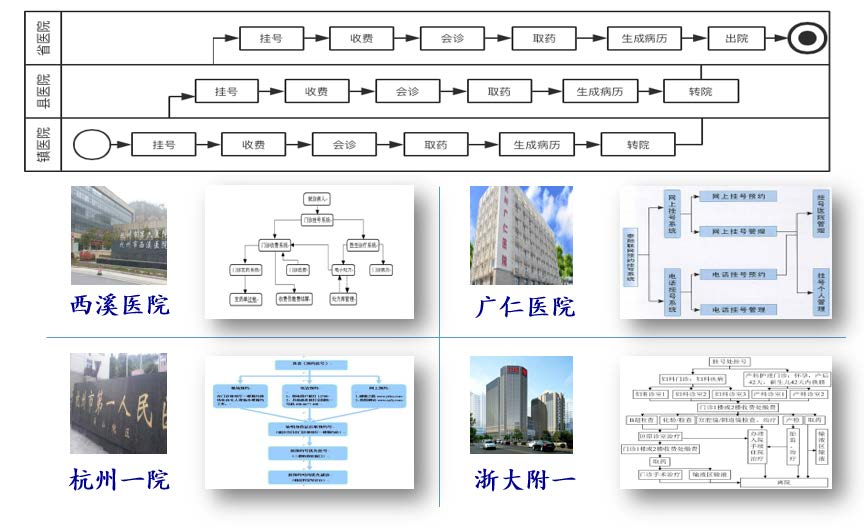
\includegraphics[scale=1]{./images/hospitalRunningModel.jpg}
  \caption{传统医院经营模式下,各家医院标准不一}
  \label{fig:hospitalRunningModel}
\end{figure}

首先,Web API 的描述问题:许多Web API 缺乏有效的描述文档,这给其使用者带来
了很大的障碍。另外,Web API 缺乏统一的描述规范,导致各个公司、组织等都在使用自定
义的、不一致的描述方式,这对于各企业、组织间Web API 的集成和交互式非常不利的,如图\ref{fig:hospitalRunningModel}所展示的,各个地方的医院系统标准不一。再
有就是现在的Web API 描述文档,都是针对人类用户的,缺乏机器可理解性,这对于Web
API 的高效应用,诸如自动组合等方面都是很不利的。

其次,Web API 当前的使用体验问题:用户需要仔细阅读相应的说明文档,然后往往
还需要根据所提供的Web API 的请求和响应等,结合自己的实际需要,进行一层定制或者
包装工作,要正确的使用一个Web API 来获得满足自己需求的结果其实并不容易。

然后,Web API 的选择问题:在很多功能类似的服务中选择一个合适的对很多用户来
说是个挑战。

最后,Web API 的演化问题:服务提供者经常需要升级他们的服务,尽管他们力求做
到向后兼容,但往往还是会或多或少的破坏原来的Web API 接口,服务使用者不得不被迫
修改他们的应用代码以适应新的Web API 的要求,这经常是一项枯燥又繁琐的工作。

本文从服务使用者的角度出发,为解决上述Web API 使用过程中的问题,提出了服务
映射的方法,并开发了相应的系统来支持用户更好的使用服务。

\section{研究意义}
现代服务业是中国经济发展战略中的重要组成部分,也是衡量一个国家经济发展水平
的重要标志。推动现代服务业的发展壮大已成为当前中国经济发展的重要目标和关键动力。
服务计算作为现代服务业发展的重要技术基础,需要结合现代服务业发展的具体场景和具
体问题进行深入的研究和应用。同时,近年来,数字经济已成为全球经济的重要驱动力,“工业+技术”的无限融合不断为市场经济注入新的动力。
在这一发展的浪潮中,企业将大多数业务以Web服务的形式部署在网络中,并为实现复杂业务提供了最基本的功能单元。
最初,这种复杂的业务模型通常是在企业内部实现的,即不同部门根据预定的任务划分提供自己的服务,最终实现复杂而完整的产品。 
但是,随着开发人员要求日益复杂和全球分工明确,单个企业可以提供的服务将不再能满足市场需求。 因此,需要跨企业边界的服务流程来实现业务增值。

本文依托于国家重点研发计划专项《现代服务业共性关键
技术研发及应用示范》的子课题《跨界服务集成方法与支撑载体》,围绕在研究跨界服务集
成和交互过程中发现的Web API 描述文档缺乏、描述方式不一致等导致的集成困难、难以
交互,以及服务使用者使用Web API 过程中遇到的门槛较高、难以上手,需要根据自身需
求进行包装和定制操作,同类服务难以选择,以及Web API 演化导致的应用失败等实际问
题进行了深入的研究和分析,提出了一套以服务映射为基础的解决方案,并
开发了对应的原型系统,不但能够有效解决跨系统的Web API 集成问题,而且提出了以用户为中心的Web API 的使用方式,能够大大简化和改善用户使用Web API 的流程和体验,
还能够避免Web API 演化带来的应用失败的问题,因此本文的研究具有重要的意义。如图\ref{fig:yilianti}
所示,医联体环境下医院经营模式,集成了海量的服务,对用户暴露统一的接口,大大简化了用户的操作。



具体来说,对于一个大型的跨界服务接入平台,当接入的服务数量到达一定阈值时,会出现大量同类型的服务重复接入的情况,比如每一家医院
都有自己的药品查询服务,这一类服务每家医院的名称可能不同,参数可能略有差异,但输入的语义信息都十分接近,可以看作同质服务,
随着接入医院数量的增多,这无疑是一件繁琐且冗余的工作,增加了开发人员的负担而且会有程序漏洞的风险;而且,每个具体的服务参数不同,
对于用户来说,同类型服务下每一个服务就要输入一组参数,而这些参数往往差异不大,简化用户操作无疑势在必行。基于此,
我们提出了服务映射的概念,对于某一类型的服务,在平台内部提出标准服务的概念,标准服务有自己的属性和参数,可在平台内运行,
将该类型同质异构服务自动映射到标准服务,从而快速接入服务,去除繁琐的冗余工作,节约开发成本,
对外暴露统一的标准服务,方便用户,提升用户体验,用户在调用执行标准服务时系统自动映射到实体服务中。

\begin{figure}[htbp]
  \centering
  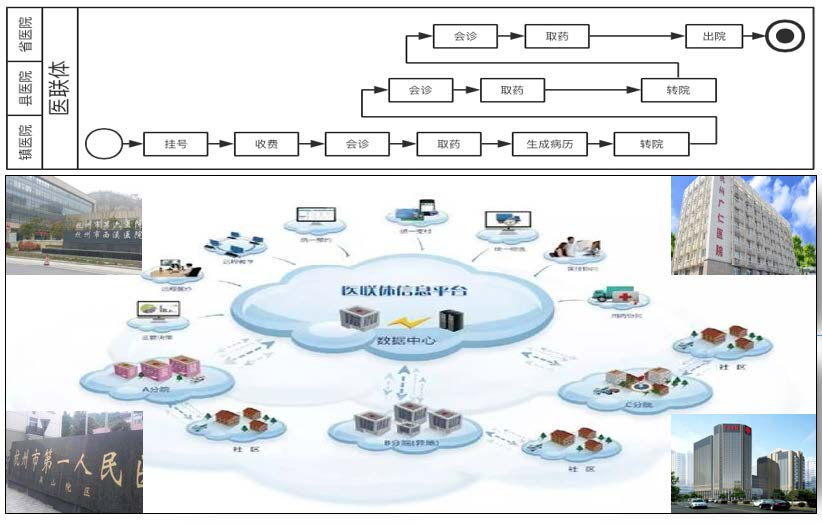
\includegraphics[scale=1]{./images/yilianti.jpg}
  \caption{医联体环境下医院经营模式图}
  \label{fig:yilianti}
\end{figure}

 同时,在当前情况下,当企业想要实施复杂的业务时,如果没有单个Web服务可以满足用户所需的功能,则应该有可能将现有服务组合在一起以满足请求。
 首先需要分析如何将业务划分为几个模块,
 以及每个模块需要什么原子服务。之后,他需要构建服务流程并基于QoS进行服务选择。
 上述两个步骤中的每一个都十分繁琐,并且需要非常丰富的领域专家知识。显而易见,对于这样的一个个流程,当数量达到
 一定阈值时,也会出现上述和标准服务一样的问题:各个服务流程提供商对解决的同一问题呈现出了不同的流程细节,
随着接入流程提供商数量的增多,这无疑是一件繁琐且冗余的工作,增加了开发人员的负担而且会有程序漏洞的风险;而且,每个具体的流程参数、步骤不同,
对于用户来说,同类型流程下每一个服务就要输入一组参数,而这些参数往往差异不大,简化用户操作无疑势在必行。
 本文将同类型(同质)实体流程抽象为标准流程作为统一解决方案,例如医院要发布一站式在线挂号服务的情况,
 该需求大体可以通过“部门信息获取”,“专家信息获取”,
 “注册资源获取”,“注册”和“账单支付”五个功能模块(子服务)对整个业务的服务流程进行建模,可将此作为标准流程构建在跨界
 服务平台。从而实现快速接入流程,去除繁琐的冗余工作,节约开发成本,
 对外暴露统一的标准流程,方便用户,提升用户体验,用户在调用执行标准流程时系统自动映射到实体流程中。


\section{国内外研究现状}

“云大物移智”等新一代信息技术的发展与应用,使得人类的认知扩大、能力增强,
也将重新定义传统边界。“跨界”即突破原有界限,实现界内和界外资源的整合与协作。
跨界服务将跨越不同行业、组织、价值链等边界的服务进行深度融合和模式创新,为用
户提供多维度、高质量、富价值服务,这不仅是技术发展的必然,也是现代服务业发展
的重要创新途径。

相比传统的服务集成,跨界服务融合需开展模式、生态、环境、质量、价值等多维
深度融合,具有极大挑战。目前国内外依然缺少跨界服务本质规模与模式认知、设计与
管理方法、质量管理与价值工程等方面的系统研究,也缺少相关工程方法和支撑载体。
从以下四个方面综述国内外的相关研究:

(1) 服务模式创新是推动现代服务业快速发展的重要因素。近年来,国际上出现
了以Artifact 为中心的商业流程建模方法、基于商业交易过程的商业模式分析框架等,
对服务模式进行了分析和建模;国内浙江大学首次提出了跨界服务概念及其3C 特点。
但总体来看,目前学术界在跨界服务本质规律认知、模式定量分析与评估等方面仍处于
探索阶段。

(2) 跨界服务设计关注如何获取和分析角色多元的用户真实需求,并根据用户需
求进行服务架构、流程和接口等生态设计。IBM 研究院、北京大学、武汉大学等单位的
研究团队在服务需求建模、服务设计和服务互操作性管理等方面具有较好的研究积累,
做出了一系列代表性工作如SOMA-ME、RGPS 需求元建模框架、基于Tropos 的服务建模
方法等,但针对跨界服务融合的设计目前仍缺少完整、系统的支撑方法体系。

(3) 跨界服务融合需要高效、可靠的运行支撑环境,以提供服务网络的运行态支
持。目前这一领域主要有企业服务总线、企业应用集成等相关技术,北京大学、IBM、
佐治亚理工学院等在云端融合资源服务化、服务总线等方面具有较好研究积累,但这些
技术大多针对企业级运行环境,仅实现服务的结构和信息融合,难以应对跨界服务所需
的多维深度融合、动态服务网络优化、开放环境安全管控等挑战。

(4)对服务系统进行精准的能力配置以提供特定的质量与价值,并在运行时准确
感知它们的实际提供水平以做出调控和改进。IBM 研究院、荷兰阿姆斯特丹自由大学、
哈尔滨工业大学等单位的研究团队在服务质量设计与度量、服务价值建模、服务价值感
知等方面具有较好的研究积累,做出了一系列代表性工作,如VASEM、服务价值网等,
但针对跨界服务质量体系和价值工程的研究仍处于初期阶段。

\begin{table}[htb]
  \centering
  \caption{国外从事相关研究的主要机构}
  \label{tab:RelatedResearchAbroad}
    \begin{tabular}{p{4cm}|p{4cm}|p{6cm}}
      \toprule
      % & \multicolumn{1}{m{60mm}}{\heiti\centering 相关研究成果}
      \multicolumn{1}{l|}{\heiti 机构名称} & \multicolumn{1}{l|}{\heiti 相关研究内容} & \multicolumn{1}{l}{\heiti 相关研究成果}\\
      \midrule
      % IBM & 服务科学、服务工程;\\
      IBM & 服务科学、服务工程;& 提出了服务计算研究框架、服务科学、管理与工程体系\\ \hline
       Carnegie Mellon University & 服务测试、组合、推荐等服务计算关键技术 & 提出了服务集成模型、基于语义的服务发现、组合等方法\\ \hline
 University of Sydney & 服务交互模型、服务资源调度、服务质量管理 & 提出了服务质量预测方法、服务组合优化、服务信任度量等方法\\ \hline
 Cambridge Service Alliance,UK & 复杂服务系统、服务使能技术方法&提出了数据驱动复杂业务建模、复杂服务网络管理等方法\\ \hline
 American Service Research & 服务设计、服务质量管理、服务化工程&提出了智能服务设计、服务创新管理等方法\\ \hline
      % \rowcolor[gray]{.9} colortbl & 表格上色。自己看着爽而已,打印出来都是黑白的。 \\
      % threeparttable & 用来给表格添加脚注啥的很方便。 \\
      % array & 忘了用来做什么了,但似乎很重要。 \\
      \bottomrule
    \end{tabular}
\end{table}

\begin{table}[htb]
  \centering
  \caption{国内从事相关研究的主要机构}
  \label{tab:RelatedResearchInChina}
    \begin{tabular}{p{2cm}|p{4cm}|p{8cm}}
      \toprule
      % & \multicolumn{1}{m{60mm}}{\heiti\centering 相关研究成果}
      \multicolumn{1}{l|}{\heiti 机构名称} & \multicolumn{1}{l|}{\heiti 相关研究内容} & \multicolumn{1}{l}{\heiti 相关研究成果}\\
      \midrule
      % IBM & 服务科学、服务工程;\\
      浙江大学 &面向现代服务业的服务计算 &在服务计算相关CCF A 类期刊、会议以及IEEE Trans 上发表论文80余篇,累计GoogleScholar引用超过5000次;获得国家发明专利100 余项。\\ \hline
      武汉大学 &软件服务工程 &主持研制5 项软件服务 相关ISO 国际标准(已 颁布),在IEEE Transactions on Services Computing 和 ICWS 等期刊和会议发 表30 余篇相关论文。\\ \hline
      哈尔滨工业大学 &服务价值工程、 服务质量管理 &提出了价值知觉的服 务工程方法体系,在 IEEE Transactions on Services Computing 和 ICWS,、ICSOC 等相关期 刊和会议上发表30 余 篇相关论文。\\ \hline
      北京邮电大学 &网络服务与智能服务平台 &在IEEE/ACM Transactions 期刊和 CCF A 类会议上发表学 术论文50 余篇,ESI 高 被引文章4 篇,获得国 家发明专利60 余项。\\ \hline
      阿里研究院& 电子商务服务及服务中间件& 探索了电商服务模式,研究数据时代的经济范式,制定了电商服务支撑平台的若干标准,突破了服务组合、服务流程、服务导出等相关的关键技术。\\ \hline
      % \rowcolor[gray]{.9} colortbl & 表格上色。自己看着爽而已,打印出来都是黑白的。 \\
      % threeparttable & 用来给表格添加脚注啥的很方便。 \\
      % array & 忘了用来做什么了,但似乎很重要。 \\
      \bottomrule
    \end{tabular}
\end{table}



关于本文的主要论点:参考服务与参考流程,即服务的映射问题和流程的映射问题,是本文提出的创新性论点
目前国内外暂时没有找到相关研究,但下文会提到,本文把服务和流程的映射问题转化为了nlp领域相对较为成熟
的命名实体识别问题,因此本节接下来简要介绍一下关于命名实体识别的国内外研究状况。

命名实体识别(NER)的任务是识别文本范围内提及的命名实体,并将其分类为预定义的类别,
例如人名,位置,组织等。命名实体是一个单词或短语,
命名实体的示例包括一般域中的组织名称,人员名称和位置名称,生物医学领域中的基因,蛋白质,药物和疾病名称,
NER是将文本中的命名实体定位和分类为预定义实体类别的过程,如图\ref{fig:nerp2}。NER充当各种自然语言应用程序(例如问答系统,文本摘要和机器翻译)的基础。
尽管早期基于统计规则的NER系统成功地产生了不错的识别精度,但是在精心设计规则或功能时,它们通常需要大量的人工。
近年来,通过连续实值矢量表示和通过非线性处理的语义合成的支持,深度学习已被应用于NER系统中,从而产生了最优异的性能。

NER的演变过程,如图\ref{fig:nerp}所示:MUC-6首次使用“命名实体”(NE),
其任务是识别文本中的组织名称,人名和地理位置以及货币,时间和百分比表达式。
自从MUC-6以来,人们对NER的兴趣越来越高,各种测评任务为此主题投入了很多精力。关于问题的定义,
Petasis等限制了命名实体的定义:“ NE是专有名词,充当某物或某人的名称”\cite{petasis2000automatic},
关于NER中应用的技术,主流方法主要有四种:1)基于规则的方法,由于它们依赖手工制定的规则,因此不需要带标注的数据; 
2)无监督学习方法,该方法依靠无监督算法而无需手工标记训练样本; 3)基于特征的监督学习方法,该方法依赖于监督学习算法并经过精心的特征设计; 
4)基于深度学习的方法,该方法以端到端的方式自动从原始输入中发现分类和检测所需的表示形式(特征)。

\begin{figure}[htbp]
  \centering
  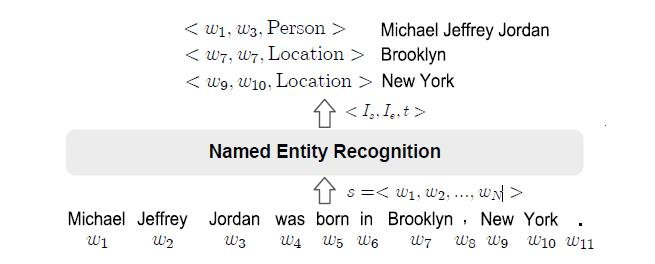
\includegraphics[scale=1]{./images/nerp2.jpg}
  \caption{命名实体识别流程}
  \label{fig:nerp2}
\end{figure}

\begin{figure}[htbp]
  \centering
  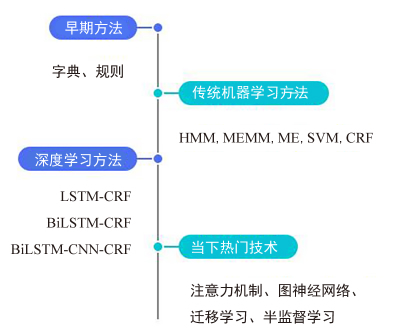
\includegraphics[scale=1]{./images/nerp.jpg}
  \caption{命名实体识别技术研究发展趋势}
  \label{fig:nerp}
\end{figure}

\subsection{基于统计规则的方法}

基于规则的NER系统依赖于人工手动制定的规则,可以基于特定领域的地名词典和句法词法模式设计规则。
Kim等提出使用布里尔规则推理方法进行语音输入,该系统会根据Brill的语音标记器自动生成规则\cite{kim2000rule}。
在生物医学领域,Hanisch等提出了ProMiner,它利用预处理的同义词词典来识别生物医学文本中提及的蛋白质和潜在基因\cite{hanisch2005prominer}。 
Quimbaya等出了一种基于字典的电子健康记录中NER的方法\cite{pomares2016named}。
实验结果表明,该方法在对精度的影响有限的前提下可提高召回率。
其他一些基于规则的知名NER系统包括LaSIE-II,NetOwl,Facile,SAR,FASTUS和LTG系统。
这些系统主要基于手工制定的语义和语法规则来识别实体。当词汇详尽无穷时,基于规则的系统可以很好地工作。
但是,由于特定领域的定制规则和不完整的词典,此类系统中经常会出现高准确率和低召回率的现象,并且这些系统无法很好到迁移到其他域。

\subsection{无监督学习方法}

无监督学习的一种典型方法是聚类,基于聚类的NER系统根据上下文相似性从聚类类簇中提取命名实体,
其核心思想是,可以使用在大型语料库上计算出的词汇资源,词汇模式和统计信息来推断命名实体。 
Collins等观察到,使用未标记的数据将对监督的要求减少到仅需7个简单的“种子”规则\cite{collins1999unsupervised},
然后,作者提出了两种用于命名实体分类的无监督算法。类似地,Etzioni等利用一组谓词名称作为输入,并利用一小组通用提取模式中实现其识别过程\cite{etzioni2005unsupervised}。 
Nadeau等提出了一个非监督系统的地名词典建设和命名实体歧义解决方案,该系统基于简单而高效的启发式方法,结合了实体提取和歧义消除功能\cite{nadeau2006unsupervised}。
另外,Zhang和Elhadad提出了一种从生物医学文本中提取命名实体的无监督方法\cite{zhang2013unsupervised},
他们的模型不是监督,而是求助于术语,语料库统计信息(例如逆文档频率和上下文向量)和浅层语法知识(例如名词短语分块),
在两个主流生物医学数据集上进行的实验证明了其无监督方法的有效性和可推广性。

\subsection{基于特征的监督学习方法}

通过监督学习,NER被转换为多类别分类或序列标记任务。给定带标注的数据样本,特征经过精心设计以能够代表每个训练示例。
然后,利用机器学习算法来学习模型,以从未标注数据中识别出相似的模式。特征工程在有监督的NER系统中至关重要,
特征向量表示是对文本的抽象,其中一个或多个布尔值,数字值代表一个单词。单词级功能(例如大小写,词法和词性标记),
列表查找功能(例如Wikipedia地名词典和DBpedia地名词典),
以及文档和语料库特征(例如,本地语法和多次出现)已广泛用于各种有监督的NER系统。
许多机器学习算法已应用于有监督的NER,包括隐马尔可夫模型(HMM),决策树,最大熵模型,支持向量机(SVM)
和条件随机场(CRF)。 Bikel等提出了第一个基于HMM的NER系统,名为IdentiFinder,用于识别和分类名称,
日期,时间表达式和数字量\cite{bikel1998nymble,bikel1999algorithm}。此外,Szarvas等通过使用C4.5决策树和AdaBoostM1学习算法开发了一种多语言NER系统。
一个主要优点是,它提供了一种可能即可以通过功能的不同子集训练几个独立的决策树分类器,然后通过多数表决方案组合其决策\cite{szarvas2006multilingual}。 
Borthwick等通过应用最大熵理论提出了“最大熵命名实体”(MENE),MENE能够在做出标记决策时利用各种知识资源。
 McNamee和Mayfield使用了1000种与语言相关的功能和258种拼字法和标点功能来训练SVM分类器,每个分类器都会做出二进制决定,即当前令牌是否属于八个类之一\cite{mcnamee2002entity}。
 在预测实体标签时,SVM不考虑相邻词,CRF则考虑了上下文。 
 McCallum和Li提出了NER中CRF的特征归纳方法,在CoNLL03上进行了实验,英文成绩达到了84.04%\cite{mccallum2003early}。 
 Krishnan和Manning提出了一种基于两个耦合CRF分类器的两阶段方法,第二个CRF利用从第一个CRF的输出中得出的潜在表示\cite{krishnan2006effective}。
 此外基于CRF的NER已广泛应用于各个领域的文本,包括生物医学文本和化学文本等。

 \subsection{深度学习方法}

 近年来,基于DL的NER模型逐渐占据主导地位,并取得了最优异的成果,与基于特征的方法相比,深度学习有助于自动发现隐藏的特征。 
 将深度学习技术应用于NER有三个核心优势。首先,NER受益于非线性变换,该变换生成从输入到输出的非线性映射。
 与线性模型(例如对数线性HMM和线性链CRF)相比,基于DL的模型能够通过非线性激活函数从数据中学习复杂的特征。
 其次,深度学习为设计NER特诊节省了大量精力,传统的基于特征的方法需要大量的工程技术和领域专业知识,
 另一方面,基于DL的模型可有效地从原始数据中自动学习有用的表示形式和潜在因素。
 第三,可以通过梯度下降在端到端范式中训练深度神经NER模型,此特性使我们能够设计复杂的NER系统。
 总体的架构如图\ref{fig:nerDL}所示,
 输入的分布式表示形式考虑了单词和字符级别的嵌入,现有的分类法基于字符级编码器,单词级编码器和标签解码器,以及结合了对功能有效的POS标签和地名词典等附加功能,
 上下文编码器将使用CNN,RNN或其他网络捕获上下文相关性,标签解码器为输入序列中的token预测标签。
 例如,在图\ref{fig:nerDL}中,每个token都被预测为带有其类型的命名实体:即带有B-(开头),I-(内部),E-(结束),S-(单个),或O-(外部)的命名实体。
 当然,还有其他标记方案或标记符号,例如BIO。还可以训练标签解码器以检测实体边界,然后将检测到的文本跨度分类为实体类型。

 \begin{figure}[htbp]
  \centering
  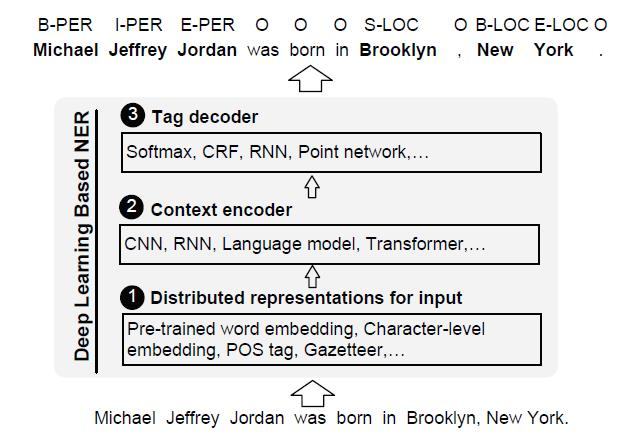
\includegraphics[scale=0.8]{./images/nerDL.jpg}
  \caption{命名实体识别深度学习方法}
  \label{fig:nerDL}
\end{figure}

BiLSTM-CRF是使用深度学习的NER最常见的体系结构。以cloze-style方式预训练双向Transformer模型的方法在CoNLL03上实现了最优异的性能(93.5%)\cite{baevski2019cloze}。 
BERT和dice loss的工作在OntoNotes5.0上达到了最优异的性能(92.07%)\cite{li2019dice}.
NER系统的成功很大程度上取决于其输入的表示形式,集成或微调预训练的语言模型嵌入正成为神经NER的研究热点,
利用这些语言模型嵌入时,可以显着提高性能。
我们从三个角度讨论利弊:输入,编码器和解码器。
首先,关于是否应该使用外部知识或如何将其集成到基于DL的NER模型尚未达成共识,
一些研究表明,外部知识可以提高NER的表现。
但是,缺点也很明显:1)获得外部知识是劳动密集型的(例如地名词典)或计算上昂贵的(例如依赖项); 2)整合外部知识会对端到端学习产生不利影响,并损害基于DL的系统的通用性。
其次,当在大型语料库上对Transformer进行预训练时,Transformer编码器比LSTM更有效。如果未预先训练且训练数据有限,则Transformer将无法完成NER任务\cite{guo2019star,yan2019tener}。
第三,RNN和Pointer Network解码器的主要缺点在于贪婪解码,这意味着当前步骤的输入需要上一步的输出。此机制可能会对速度产生重大影响,并且是并行化的障碍。 
CRF是标签解码器的最常见选择,当采用非语言模型(即非上下文化)嵌入(例如Word2vec和GloVe)时,CRF可以具有强大地捕获标签转换相关性的能力。
但是,当实体类型的数量很大时,CRF在计算上可能会很缓慢。更重要的是,当采用上下文化语言模型嵌入(例如BERT和ELMo )时,与softmax分类相比,CRF并不总是导致更好的性能。
对于最终用户,选择哪种体系结构取决于数据和域任务。如果数据丰富,则可以考虑从头开始使用RNN训练模型,并对上下文语言模型进行微调。
如果数据稀缺,则采用迁移的策略可能是更好的选择。对于新闻专线领域,有许多可用的预训练的现成模型。对于特定领域(例如,医学和社交媒体),
使用特定领域的数据对通用的上下文化语言模型进行微调通常是一种有效的方法。NER适用于不同的语言,主要关注英语和一般领域的NER。
除了英语以外,还有许多其他语言或跨语言环境的研究。
 Zhang 和 Yang 提出了一种针对中文NER的格子结构LSTM模型,该模型对输入字符序列以及与词典匹配的所有潜在单词进行编码\cite{zhang2018chinese}。
 除中文外,许多研究使用其他语言进行,包括蒙古语,捷克语,阿拉伯语,越南语,印度尼西亚语等。
 每种语言都有其自己的特征,可以理解该语言上NER任务的基础,也有许多研究旨在通过将知识从源语言转移到标签很少或没有的目标语言来解决跨语言环境中的NER问题。

迁移学习旨在通过利用从源域中学到的知识来在目标域上执行机器学习任务\cite{pan2009survey},在NLP中,迁移学习也称为领域适应。
对于NER任务,传统方法是通过自举算法。 
Pan等提出了跨域NER的转移联合嵌入(TJE)方法,TJE使用标签嵌入技术将多类别分类转换为低维潜在空间中的回归问题\cite{pan2013transfer}。 
Qu等观察到相关的命名实体类型通常共享词汇和上下文特征\cite{qu2016named},他们的方法使用两层神经网络来学习源命名实体类型和目标命名实体类型之间的相关性,
适用于源域与目标域具有相似(但不相同)的ner问题。 
Peng和Dredze在多任务学习环境中探索了迁移学习\cite{peng2016multi},他们在新闻和社交媒体这两个领域中分别考虑了:分词和NER这两项任务,
在迁移学习的设置中,不同的神经模型通常在源任务和目标任务之间共享模型参数的不同部分。
Yang等首先研究了神经网络的不同层的可迁移性\cite{yang2017transfer},然后,他们针对跨域,跨语言和跨应用程序场景提出了三种不同的参数共享架构。
如果两个任务具有可映射的标签集,则存在一个共享的CRF层,否则,每个任务将学习一个单独的CRF层。
实验结果表明,在资源匮乏的情况下(即更少的可用标签),各数据集的跑分成绩都有了显着改善。 
赵等提出了一种具有领域适应性的多任务模型,其中全连接层适用于不同的数据集,但CRF特征是分别计算的,
赵氏模型的主要优点是,在数据选择过程中会过滤掉分布不同且标注未对齐的实例\cite{zhao2018improve}。




\section{对话系统补充}
随着人工智能的飞速发展,人机对话越来越受到人们的关注。人机对话系统主要由自动语音识别(ASR),口语理解(SLU),对话管理(DM),
对话生成(DG)和文本转语音(TTS)组成[1]。意图检测作为自然语言理解的一个子模块,在提高自然语言理解和口语理解方面起着至关重要的作用。
在实际研究中,意图检测设法捕获用户的真实意图和用户的期望动作,例如饭店预订,门票预订等。
在人机对话过程中,面向任务的对话最紧急的事情要做的是获取用户的真实意图。经过一轮或多轮对话后的上下文综合判断,
可以准确捕捉用户的意图并尽快完成面向任务的对话。

传统的意图检测主要包括两种方法:基于规则的模板和基于特征的统计。基于规则的意图检测依赖于手动设置规则模板,该模板限于特定字段。 Li等。 
[3]指出,在相同的场模型下,模板的数量会由于表达式的不同而急剧增加,同时会导致制作规则模板的难度。基于特征统计的方法主要包括朴素贝叶斯(NB)[4],
Adaboost [5],支持向量机(SVM)[6]等。但是,基于规则的模板和基于特征的统计都具有难以手动提取特征,无法保证准确性。
随着深度学习的飞速发展,基于深度学习算法的意图检测应运而生。就单词向量的文本特征提取而言,Kim等人。
文献[7]将词向量分类为意图分类的词汇特征,与传统的One-hot模型相比,具有很大的性能提升。关于卷积神经网络(CNN),Hash-emi等人。 
[8]使用CNN提取文本向量作为查询特征,以识别用户的搜索意图,从而简化了特征提取过程。但是,文本的抽取意图有限,无法保留语义上的连贯性。基于递归神经网络(RNN)的LSTM解决了内存问题。基于LSTM的GRU提高了长序列保留信息的能力。两者在意图检测领域都取得了良好的进展。夏等。 [9]提出了一种基于胶囊网络的意图胶囊模型。该模型利用胶囊模型在文本建模中的优势在文本中分层构建模型。最后,本文使用基于BERT预训练的BiLSTM进行意图检测,取得了很好的效果